Le simulazioni sono state ottenute abilitando nel simulatore le componenti
corrispondenti alle seguenti flags (Il controllo di assetto è mantenuto attivo
poichè necessario per una facile interpretazione dei risultati riguardo
l'orbita poichè vengono presentati in riferimento corpo).

\begin{lstlisting}[language=matlab,breaklines=true]
GravityTypeFlag=1;		%(1=J2 Gravity Model/=0 Spherical)
GravityGradientTorqueFlag=1;	%1=Gravity Gradient Torque ON/0=OFF 
DragForceDisturbancesFlag=1;	%0=Drag Force Disturbance OFF/1=OFF
DragTorquesDisturbancesFlag=1;	%0=Drag Torque Disturbance OFF/1=ON
DragFreeControlFlag=1;		%0=Drag Free Control OFF/1=ON
AttitudeControlFlag=1;		%0=Attitude Control OFF/1=ON
\end{lstlisting}

\begin{SCfigure}[0.7][ht]
	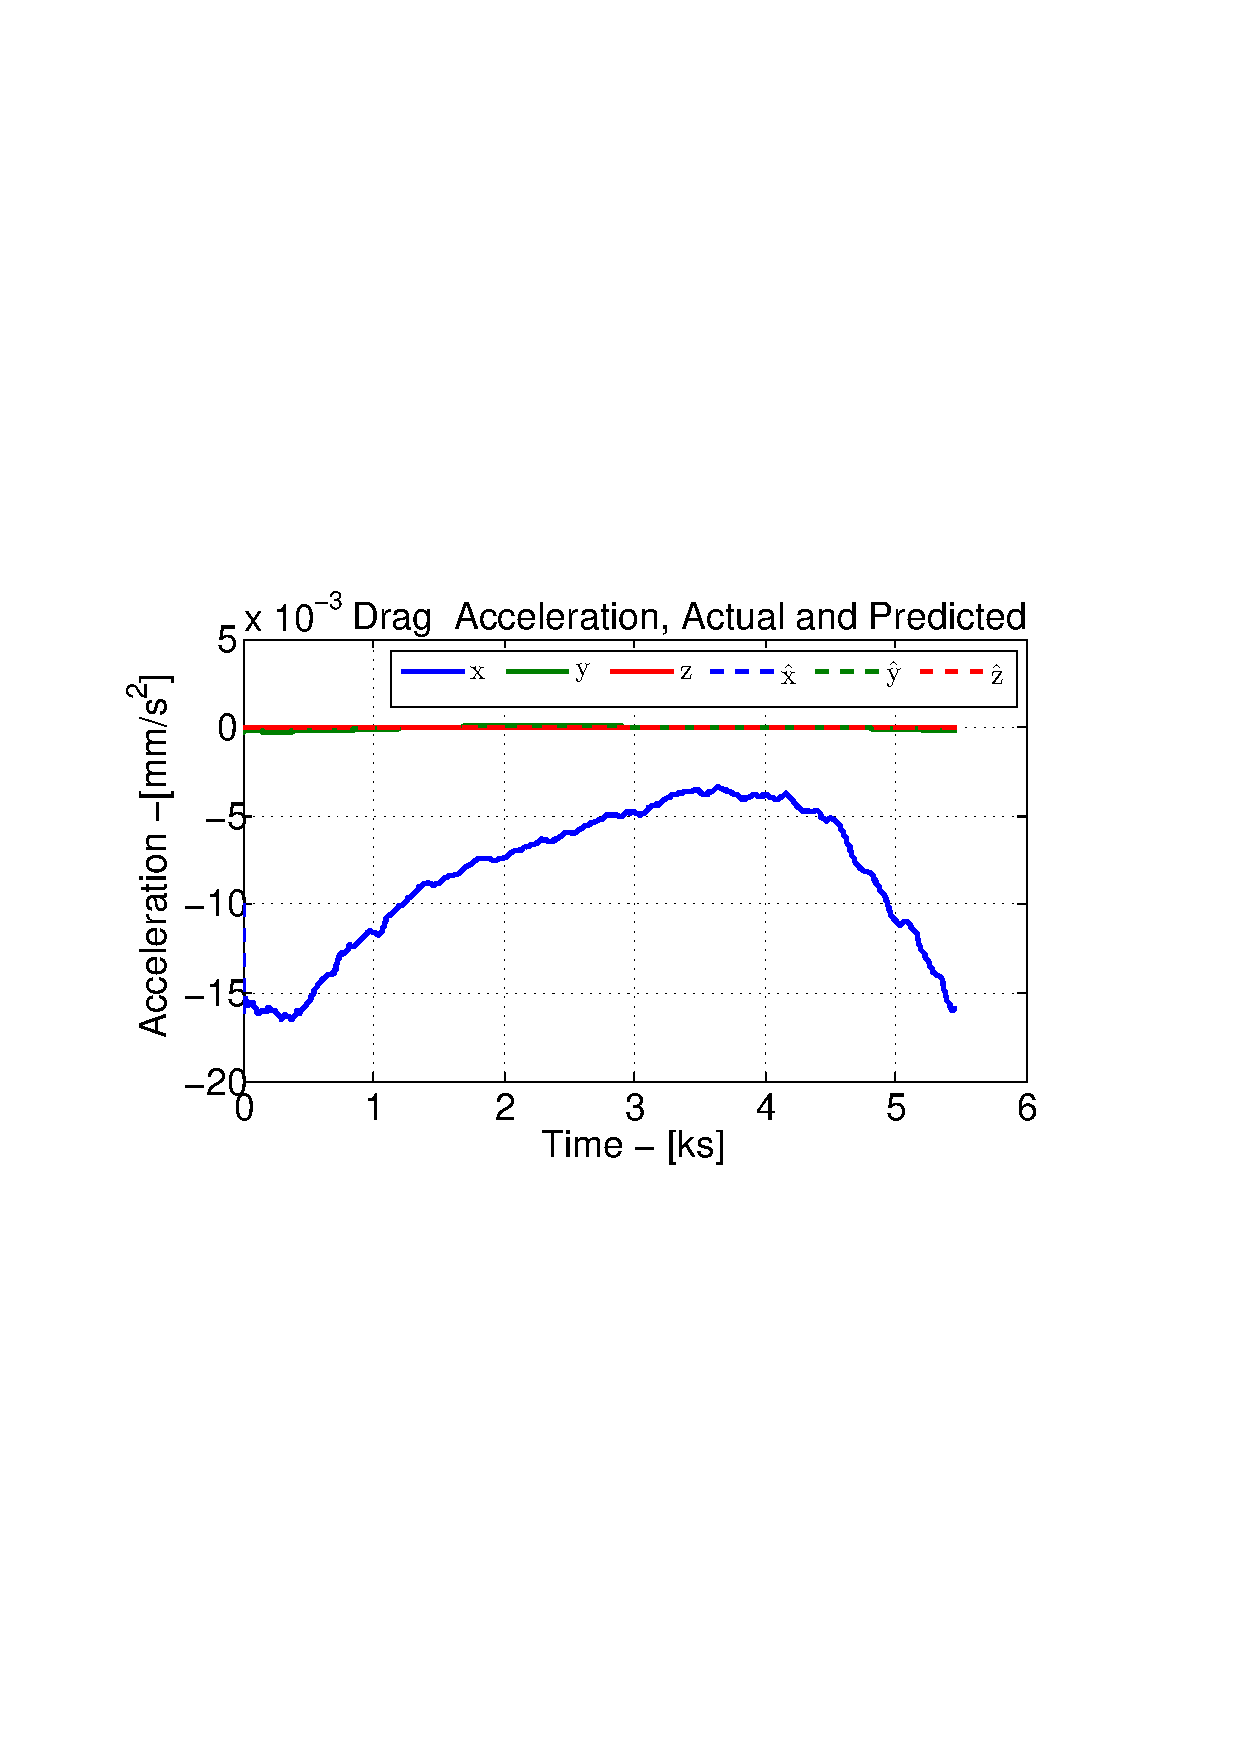
\includegraphics[width=.6\textwidth,clip=true,trim=2cm 10cm 3cm
	10cm]{control/orbit_control/images/drag_acceleration.pdf}
	\caption{\emph{Accelerazione Non Gravitazionale} --- Il predittore dello stato
	riesce a predirre l'accelerazione non gravitazionale (le curve tratteggiate a 
	questo livello di scala coincidono con 	quelle piene),  vi è una componente di
	accelerazione lungo l'asse x da compensare}
	\label{fig:drag-acceleration}
\end{SCfigure}
\begin{SCfigure}[0.7][ht]
	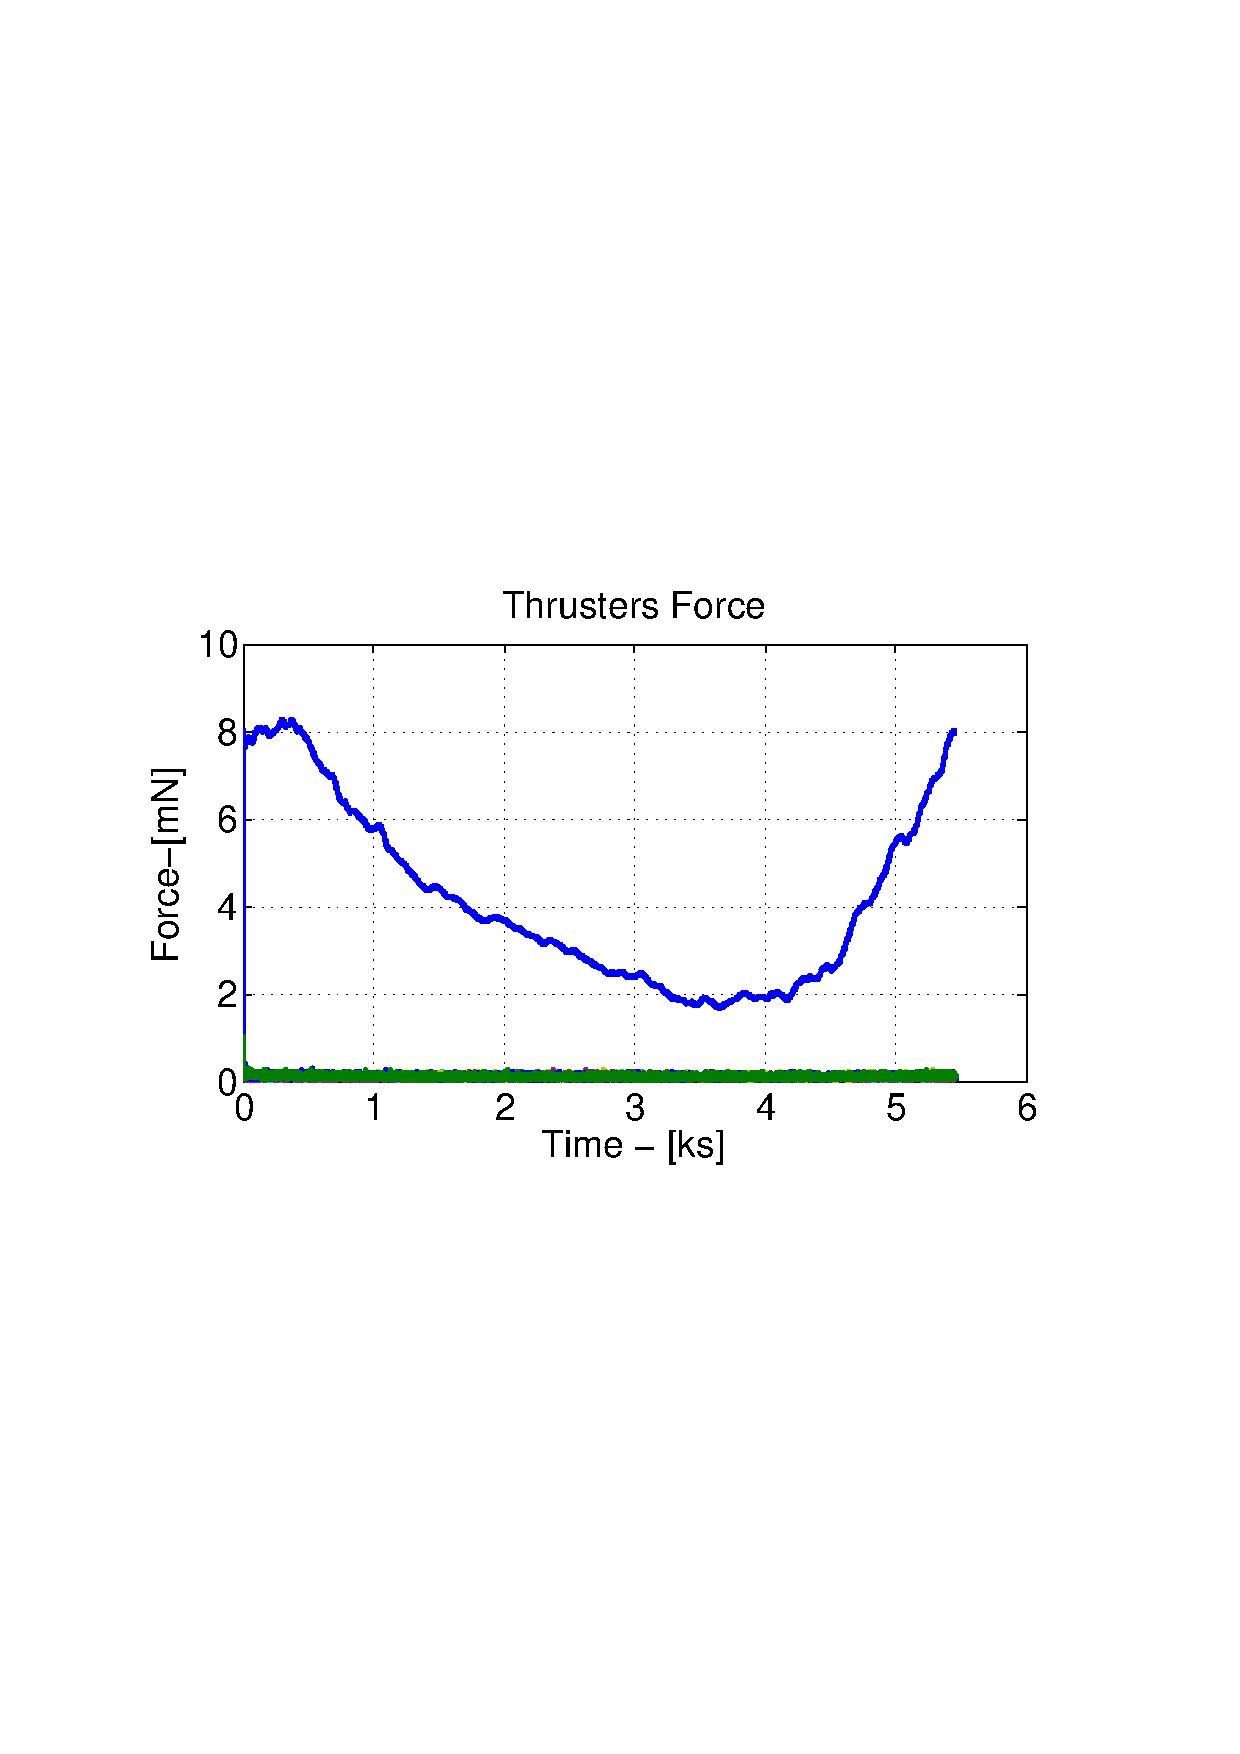
\includegraphics[width=.6\textwidth,clip=true,trim=2cm 10cm 3cm
	10cm]{control/orbit_control/images/thrusters_force.pdf}
	\caption{\emph{Forze dei propulsori} --- I propulsori compensano correttamente
	l'accelerazione non gravitazionale fornendo forze di uguale modulo ma con
	verso contrario}
	\label{fig:drag-acceleration}
\end{SCfigure}
\begin{SCfigure}[0.7][ht!]
	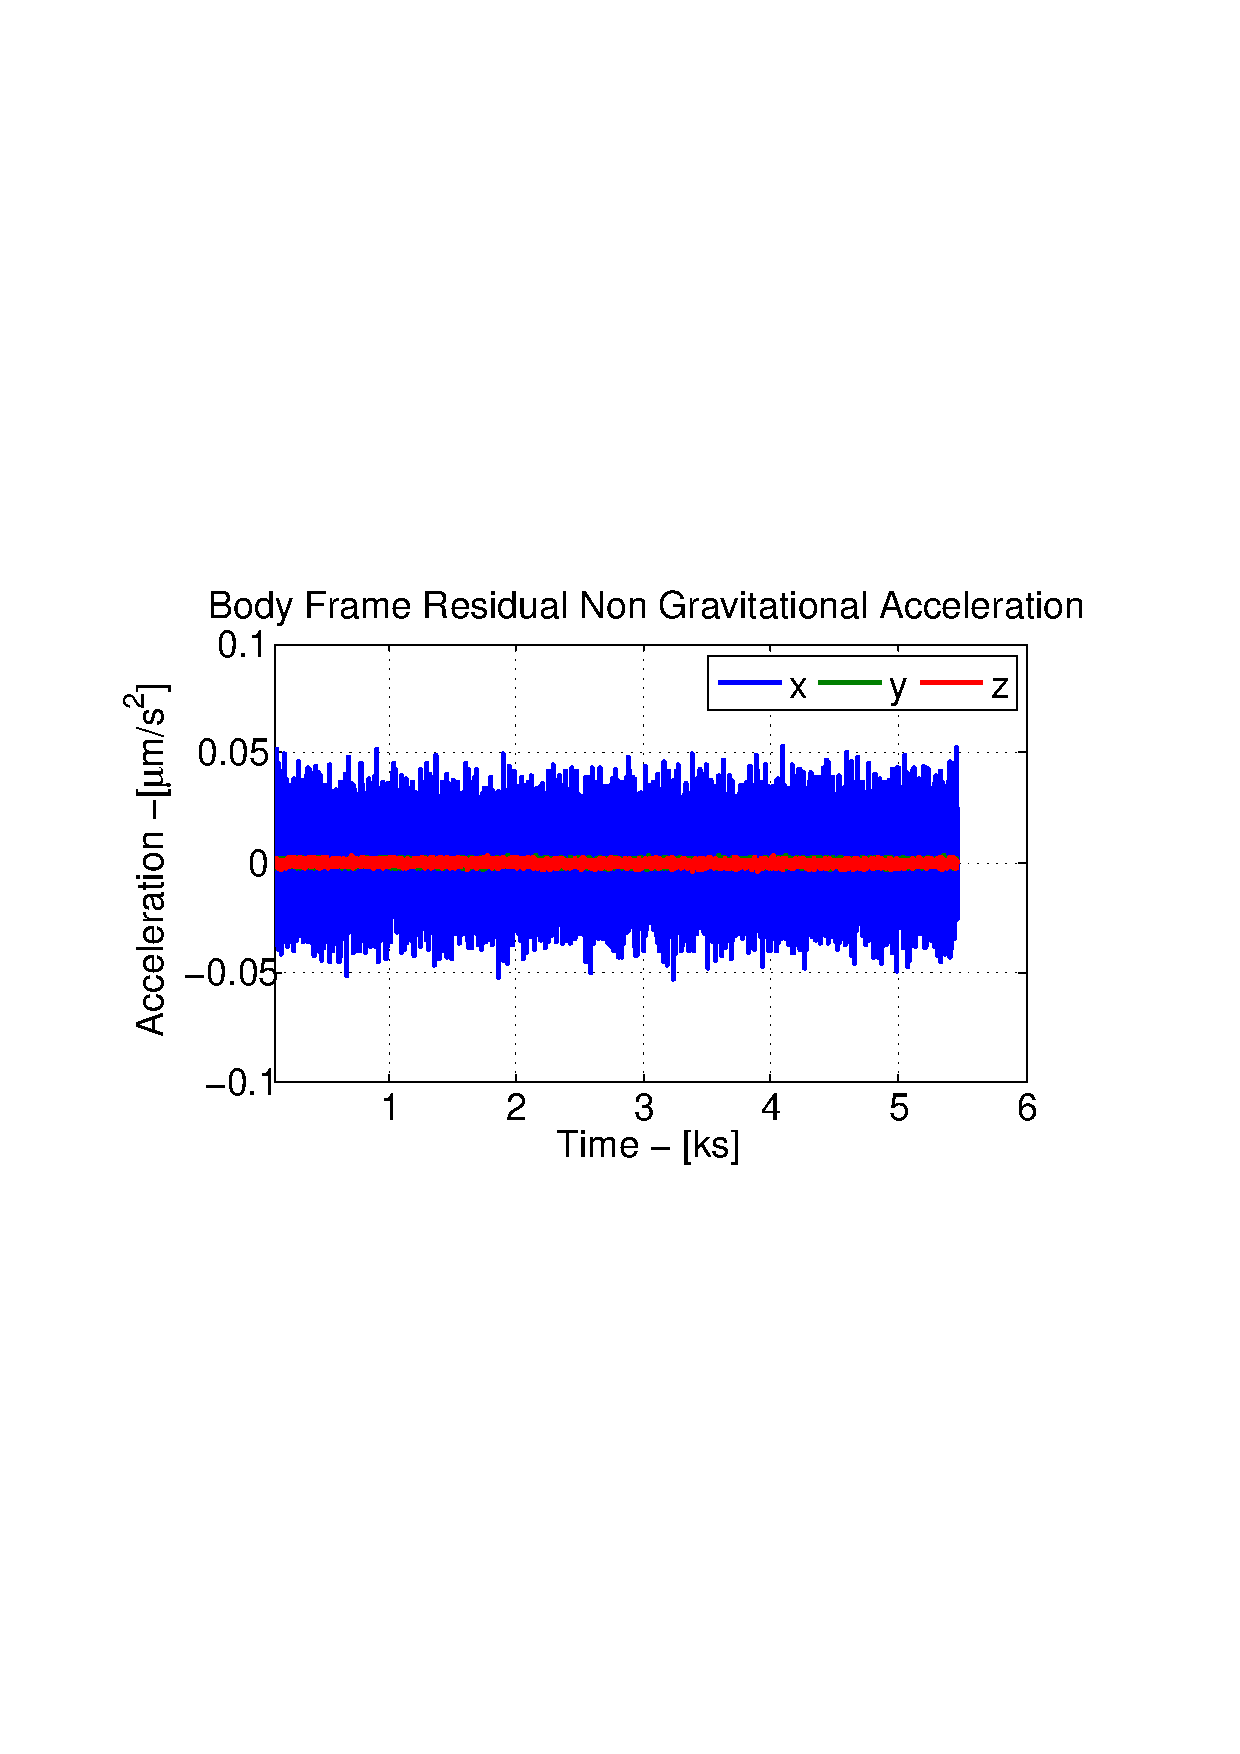
\includegraphics[width=.6\textwidth,clip=true,trim=2cm 10cm 3cm
	10cm]{control/orbit_control/images/residual_acceleration.pdf}
	\caption{\emph{Accelerazioni non gravitazionali residue in riferimento
	corpo} --- Il controllore riesce correttamente a compensare le accelerazioni
	non gravitazionali riuscendo a mantenerle nel range dei $[-0.5 \, +0.5]%
	\mu m/s^2$}
	\label{fig:drag-acceleration}
\end{SCfigure}
